\documentclass[12pt, pdflatex]{article}
\usepackage[a4paper, top=3cm, bottom=3cm, right=3cm, left=3cm]{geometry}
\usepackage[french]{babel}
\usepackage[utf8]{inputenc}
\usepackage[T1]{fontenc}
\usepackage[a4paper]{geometry}
\usepackage{amsmath}
\usepackage{graphicx} 
\usepackage{tabularx}
\usepackage{listings}
\usepackage{float}
\usepackage{caption}
\usepackage{parskip}
\usepackage{menukeys}
\usepackage{url}
\usepackage{wrapfig}
\usepackage{hyperref}


\setlength\parindent{24pt}
\newmenumacro{\nixfile}[/]{hyphenatepaths}
\newmenumacro{\nixpath}[/]{hyphenatepathswithfolder}
\newmenumacro{\winpath}[bslash]{hyphenatepathswithfolder}
\newmenumacro{\winfile}[bslash]{hyphenatepaths}


\title{Devoir de Contrôle Continu}
\author{VU Nguyen Phuong Vy}

\date{\today}

\begin{document}


\begin{titlepage}
    \centering
    
\includegraphics{sources/logo-unicaen.png}\par\vspace{1cm}
    {\scshape\LARGE Devoir de Contrôle Continu\\Complément de POO \par}
    \vspace{1cm}
    {\scshape\LARGE Jeu de Bataille Navale\par}
    \vspace{1cm}
	{\large Nguyen Phuong Vy VU - 21911658\par}
    \vspace{11cm}
    {\large L2 Informatique - Groupe 2A - Année 2020-2021\par}
	{\large \today \par}

\end{titlepage}

\pagebreak

\tableofcontents

\pagebreak
\section{Introduction}
    \subsection{Bataille Navale}

    \begin{wrapfigure}{R}{0.45\textwidth}
        \centering
        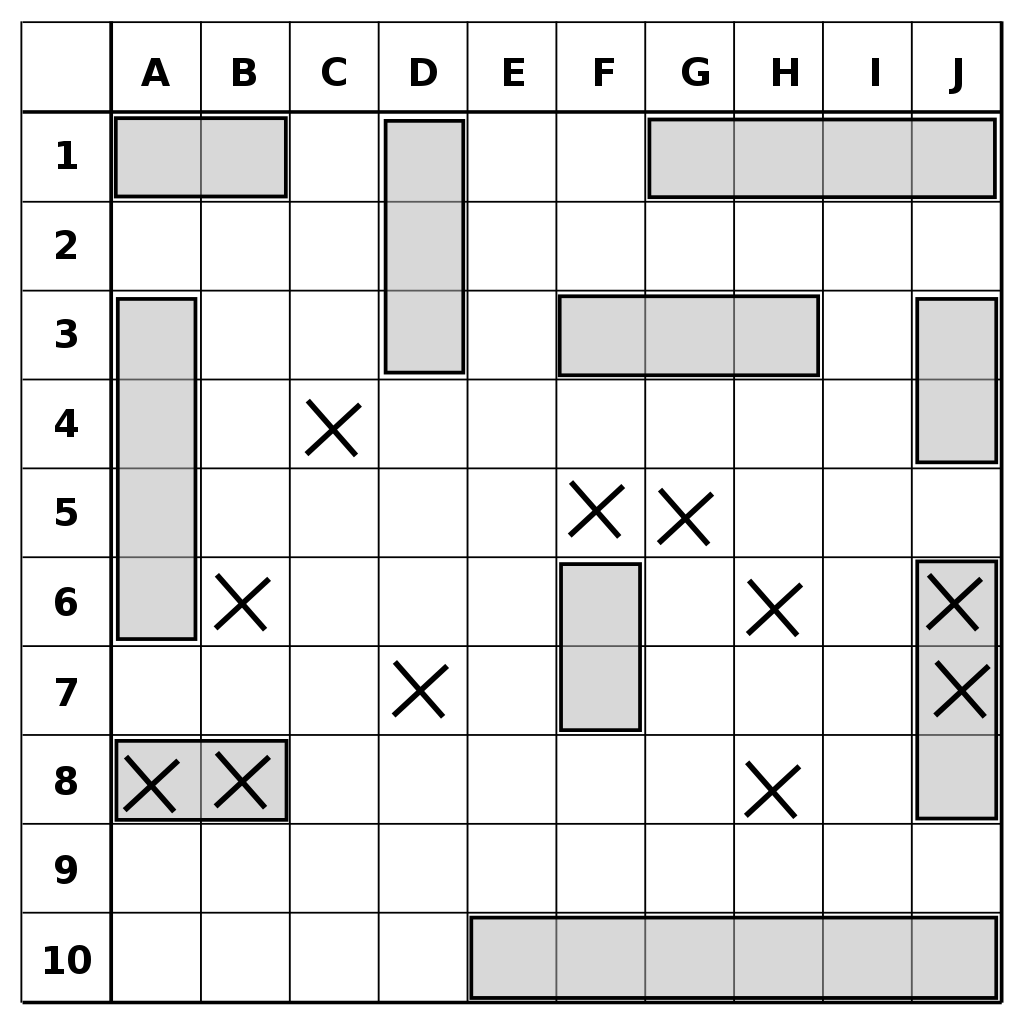
\includegraphics[width=0.4\textwidth, trim=0pt 0pt 0pt 30pt]{sources/grid.png}
        \caption{Grille du jeu}
        \vspace{-20pt}
    \end{wrapfigure}

    Bataille Navale\cite{wiki}, également appelé Touché-Coulé, est un grand classique des jeux de sociétés pour deux joueurs. Son origine est dans un jeu français "L'Attaque" au début des années 1930.

    Pour commencer ce jeu, deux joueur qui s'affrontent placer ses bateaux sur sa grille. Chacin a une flotte composée de cinq bateaux, qui sont un porte-avion, un croiseur, un contre-torpilleur, un sous-marin, un torpilleur et les bateaux ne doivent pas être collés entre eux, un navire est coulé si chacune de ses cases ont été touchées par un coup de l'adversaire.
    
    Le gagnant est celui qui ales statégies à couler tous les navires de l'adversaire avant que tous les siens ne le soient.

    \subsection{But du projet}
    Dans ce projet, on a développé un jeu avec la conception Modèle-Vue-Contrôleur (MVC) qui permet de jouer sur une interface graphique. En effet, on a lancé un planning de ce projet en plusieurs temps :

    \begin{itemize}
        \item Lancer de la conception du projet (diagramme, librairie, méthode)
        \item Développer du moteur du jeu, selon les règles du jeu
        \item Développer l'interface et le contrôleur
        \item Optimiser et vérifier le code pour éviter les bugs
    \end{itemize}

\section{Organisation du projet}
    \subsection{Hébergement du code}
    On a choisit le forge d'Unicaen pour faciliter la gestion du projet. Il permet de créer et d'administrer des dépôts sous le forge que l'on peut en faire avec terminal. De plus, le forge offre les autres fonctionnalités qui sont une gestion des permissions, une visualisation des différents commits, le suivi de l’activité du projet, etc. 

    \subsection{Tableau des tâches}
    \begin{center}
        \begin{tabular}{|p{5cm}|p{9cm}|}\hline
            \textbf{Classes}& \textbf{Tâches}\\ \hline\hline
            \textbf{Création des modèles}& \\ \hline
            Case&  Contenir un point des coordonnées et un bateau \\ \hline
            Ship&  Construire un bateaux avec un poids    \\ \hline

            \textbf{Création du plateau}& \\\hline
            Board& Construire le plateau \\ &Placer les bateaux \\ &Créer la fonction de viser  \\ \hline

            \textbf{Création de MVC}& \\\hline 
            Draw&  Dessiner l'interface graphique \\ &Viser dans le plateau avec le souris \\ \hline
            
            \textbf{Main} &Initialiser les bateaux\\ &Lancer le jeu\\\hline
            

        \end{tabular}
    \end{center}



\section{Architecture du projet}
    \subsection{Directoires du projet}
    La structure du projet est non seulement de diviser le projet en des parties spécifiques, mais encore doit adopter la structure de Gradle. Il est structuré en trois parties.

    \begin{minipage}{\textwidth}
        \begin{tabbing}
        \hspace{1em}\=\hspace{1em}\=\hspace{1em}\=\hspace{12em}\=\\\kill

        \nixpath{rapport    } \>\>\>\> \\

        \nixpath{gradle/wrapper    } \>\>\>\> \\
        
        \nixpath{src/main/java    } \>\>\>\> \+\\
        \nixpath{board  }   \>\>\>   \+\\
        \nixfile{Board.java}     \>\> \-\\

        \nixpath{model}   \>\>\>  \+\\
        \nixfile{Case.java}     \>\> \\
        \nixfile{Ship.java}     \>\>  \-\\

        \nixpath{view}   \>\>\>  \+\\
        \nixfile{ViewController.java}     \>\> \-\\

        \nixfile{Main.java}   \>\>\>  \\

        \end{tabbing}
        \end{minipage}
        \par
        On remarque les packages utilisés:
        \begin{itemize}
            \item board: initialiser le plateau avec les bateaux et les fonctions du jeu
            \item model: créer modèle du jeu
            \item view: dessiner le plateau et l'écouteur de souris
        \end{itemize}

    
    \subsection{Diagramme des classes}
    \begin{figure}[H]
        \centering
        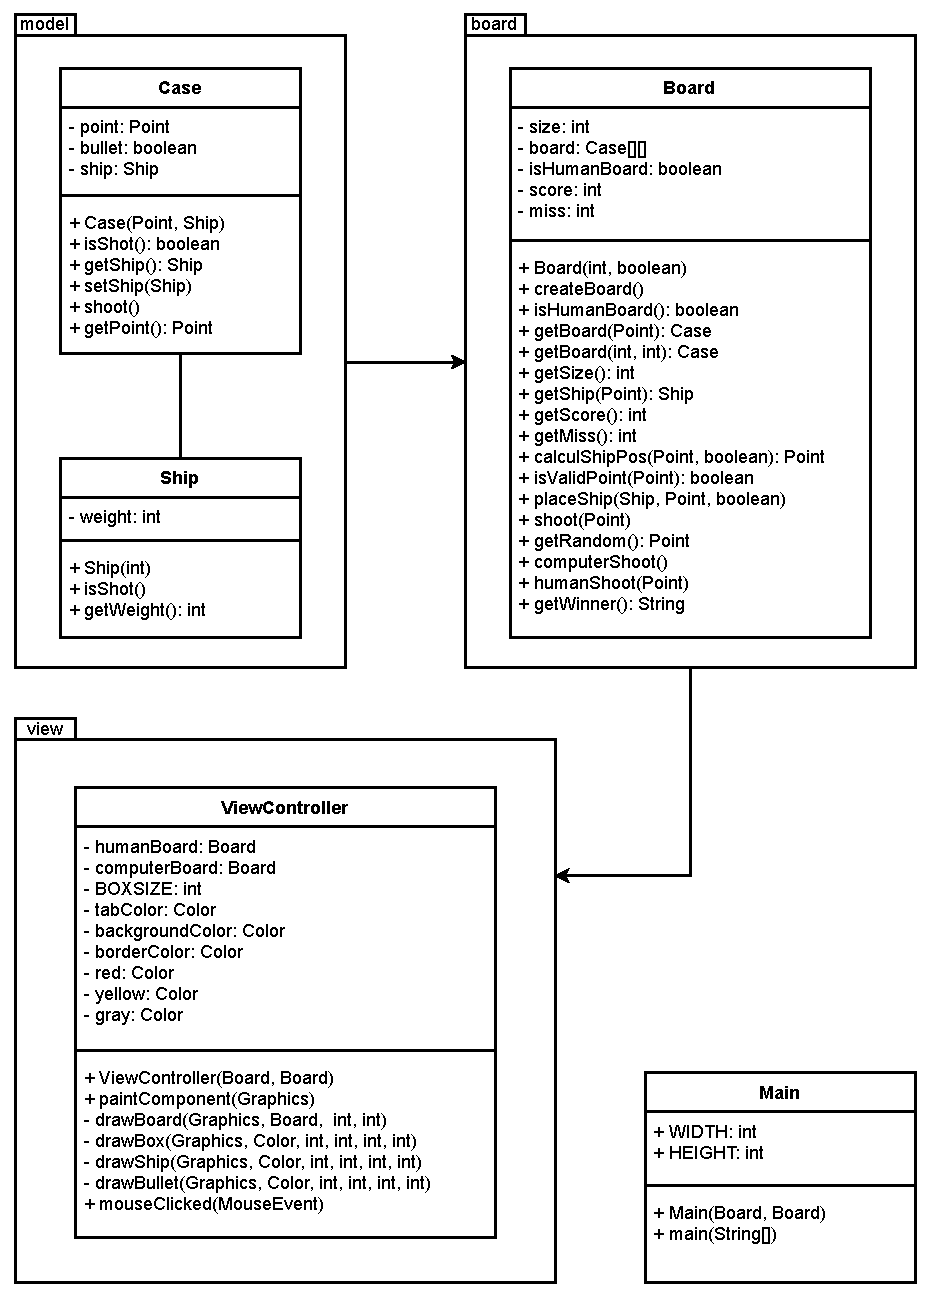
\includegraphics[width=1\textwidth]{sources/uml.pdf}
        \caption{Diagramme des classes}
    \end{figure}



\section{Développement du projet}

    \subsection{Création du plateau}
    Au début, on choisit la taille du plateau est de 10x10, 100 carrées. Donc, on crée la classe des cases nommées \textbf{Case} qui sera une petite carrée du plateau. Il y a des cases qui contiennent des bateaux ou sont nulles. On initialise les bateaux dans la classe \textbf{Ship} avec les poids et une case contient un poids du bateau.
    
    Ensuite, on construit la classe de plateau \textbf{Board} avec les cases avec le point en correspond en défaut (pas de bateau) et avec le boolean pour spécifier le plateau. Après avoir créé les cases sur le plateau, on fait une méthode de placer les bateaux \texttt{placeShip(Ship, Point, boolean)}. On note avec le boolean \texttt{true}, le bateau veut placer en vertical et vice versa, le boolean \texttt{false} est en horizontal. 

    Finalement, après avoir créé deux plateaux sur la classe \textbf{Main}, l'un de joueur et l'autre d'ordinateur. On place les bateaux sur chaque plateau.

    Ce sont des bateaux et des poids vont initialiser:
    \begin{itemize}
        \item 1 Porte-avions (poids de 5)
        \item 1 Croiseur (poids de 4)
        \item 1 Contre-torpilleurs (poids de 3)
        \item 1 Sous-marin (poids de 3)
        \item 1 Torpilleur (poids de 2)
    \end{itemize}



    \subsection{Viser sur le plateau}
    Selon aux règles du jeu, on fait la méthode de viser les bateaux par rapport au boolean des cases. Si un case est visé dont le boolean devient \texttt{true}. Quand on vise sur un bateau, le poid sera perdu et si le poid d'un bateau est de zéro, on dit ce bateau est coulé. En outre, on fait une méthode de viser par ordinateur qui utilise la classe \textbf{Random} avec le boucle pour trouver les points disponibles.



    \subsection{Design Pattern Modèle-Vue-Contrôleur (MVC)}
    Dans cette partie, on construit l'interface du jeu par la librairie Java Swing qui a été inclus au JDK depuis la version 1.2, cette libraire est moins compliquée d'installer que la librairie JavaFX, avec la conception Modèle-Vue-Contrôleur (MVC). Et on souhaite de ne pas lancer la ligne de commande quand on joue le jeu. 
    
    Java Swing\cite{swing} fait partie de la bibliothèque Java Foundation Classes (JFC). C'est un API dont le but est similaire à celui de l'API AWT, mais son fonctionnement et son utilisation sont complètement différentes.

    Modèle-Vue-Contrôleur ou MVC\cite{mvc} qui est composé de trois types de modules ayant trois responsabilités différentes : les modèles, les vues et les contrôleurs (un motif d'architecture logicielle destiné aux interfaces graphiques).

        \subsubsection{Modèle}
        Un modèle est les données à afficher. Par conséquent, on développe deux classes de modèle qui sont \textbf{Case} et \textbf{Ship}.

        \subsubsection{Vue}
        Une vue présente l'interface graphique. On dessine la grille de plateau en utilisant l'opérateur \texttt{instanceof} \textbf{Case} qui permet de tester si un objet possède, pour déterminer une carrée. On décide des bateaux coulés sont les rectangles rouge, des obus sont les cercles, les obus sur une case nulle est de couleur yellow et sur un case de bateau est de couleur rouge. On va dessiner avec les fonctions principales \texttt{fillOval} et \texttt{fillRect} de la classe \textbf{Graphics}

        En résumé, on indique les remarques de l'interface graphique sur l'image ci-dessous.
        \begin{figure}[H]
            \centering
            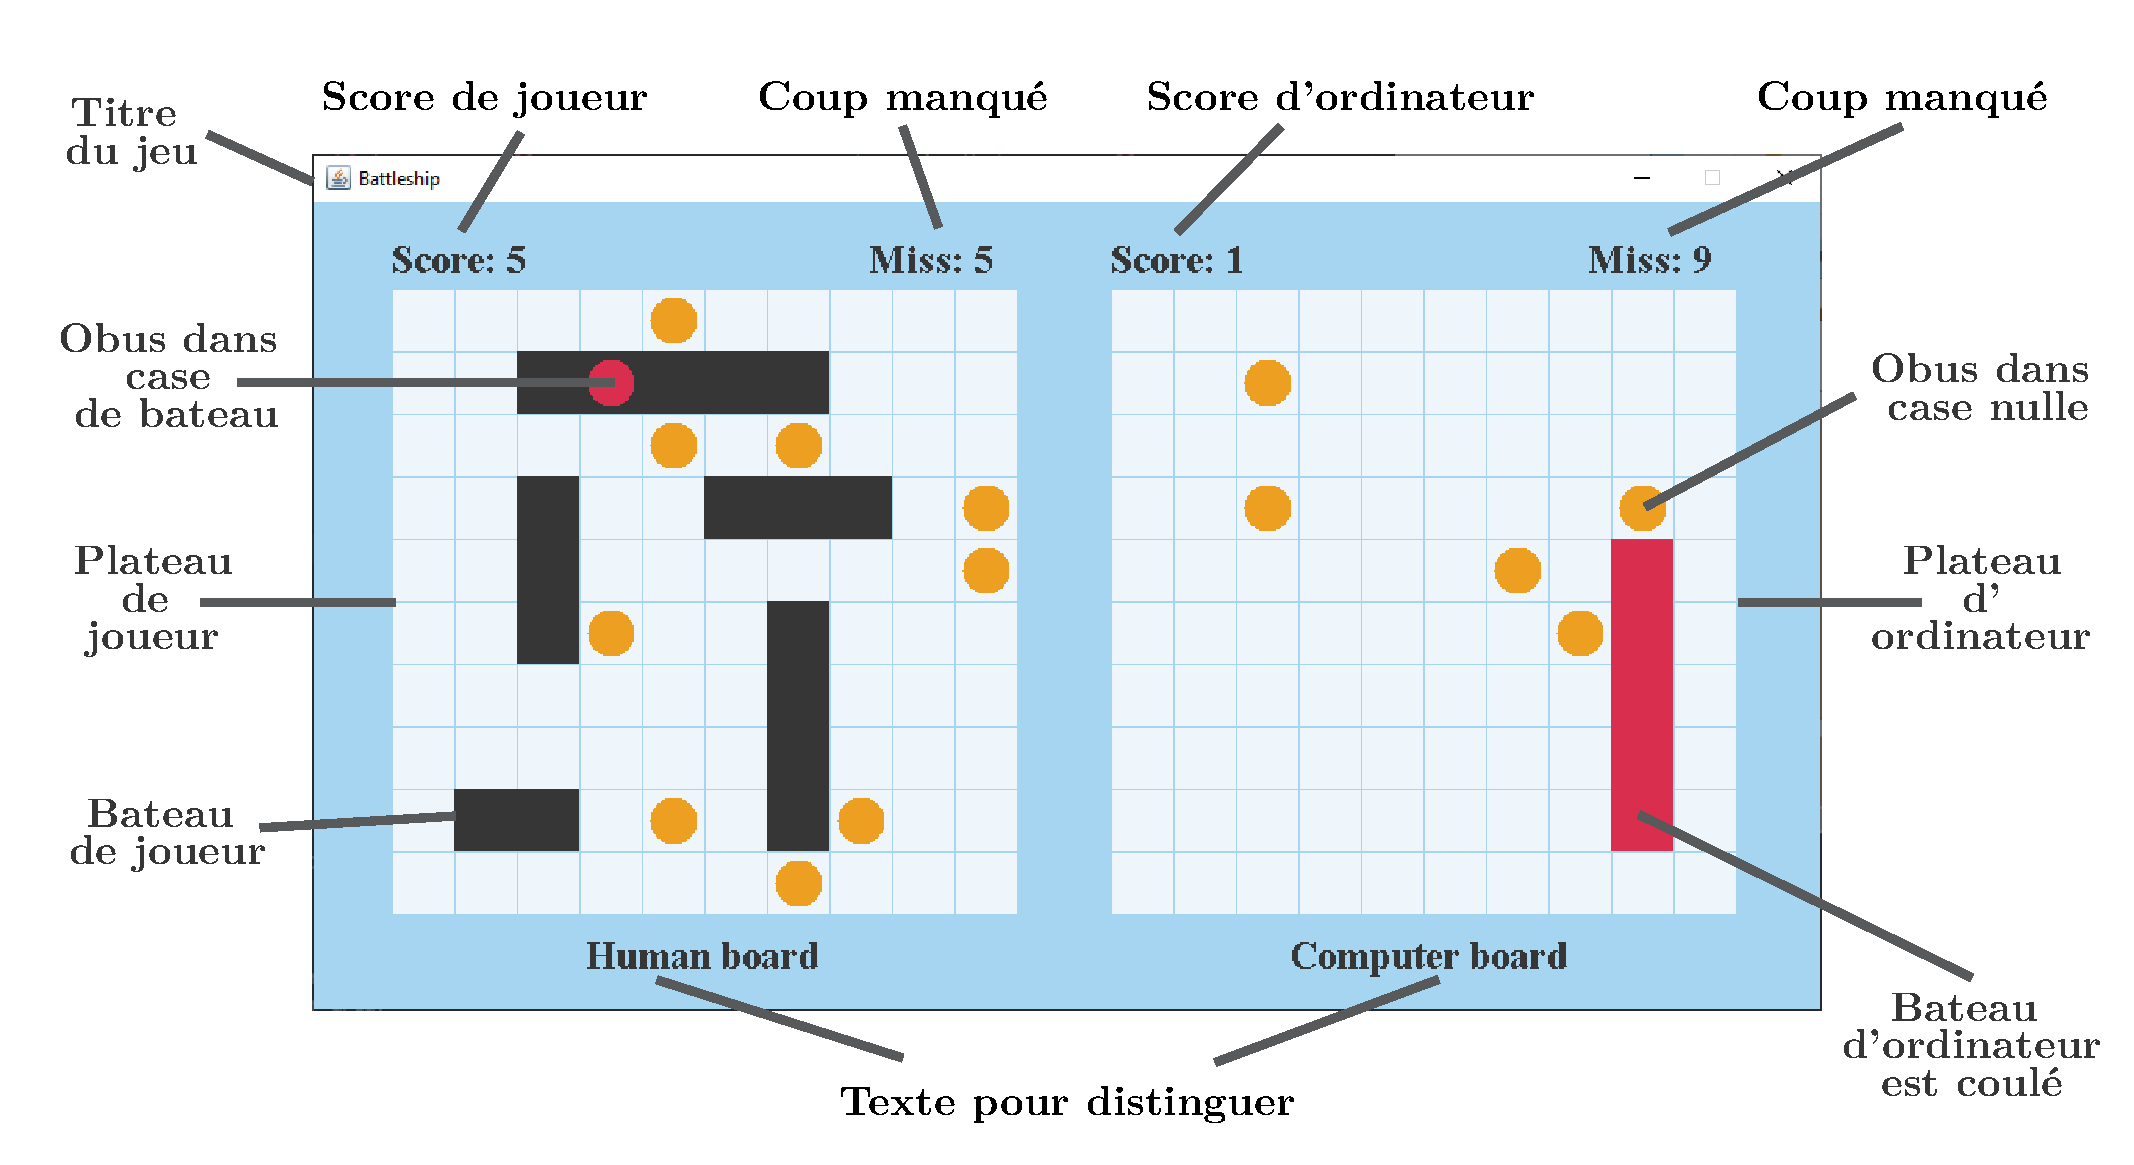
\includegraphics[width=1\textwidth]{sources/note.pdf}
            \caption{Remarques de l'interface graphique}
        \end{figure}


        \subsubsection{Contrôleur}
        Un contrôleur contient la logique concernant les actions effectuées par l'utilisateur. Pour faire les contrôleurs, on utilise l'interface \textbf{MouseListener} dans le package \textbf{java.awt.event}.

        Premièrement, on calcule le point de case par rapport les coordonnées de souris. On propose la formule pour calculer le point (x, y) de robot de la coordonnée (xPos, yPos):
        \begin{align*}
            x = (xPos - PADDING) / BOXSIZE \\ 
            y = (yPos - PADDING) / BOXSIZE
        \end{align*}

        Deuxièmement, pour viser sur le plateau avec le souris, on met les conditions des coordonnées pouvant fonctionner dans les zones autorisées de la souris et utilise la méthode \texttt{mouseClicked(MouseEvent)} pour appeler la fonction de viser.



\section{Instruction du jeu}
    \subsection{Lancer le jeu}
    Il y a beaucoup du logiciel de construction automatisée d’application qui automatisent la création d'applications exécutables à partir du code source sur la marché comme ANT, Maven et Gradle. Sur ce projet, on décide d'utiliser le Gradle, car c'est simple pour écrire le script et pour lancer.

    Entrez la commande \texttt{./gradlew run} pour lancer le jeu. Ça fonctionne avec le Linux Shell et Windows Powershell.

    \subsection{Jouer le jeu}
    
    \begin{figure}[H]
        \centering
        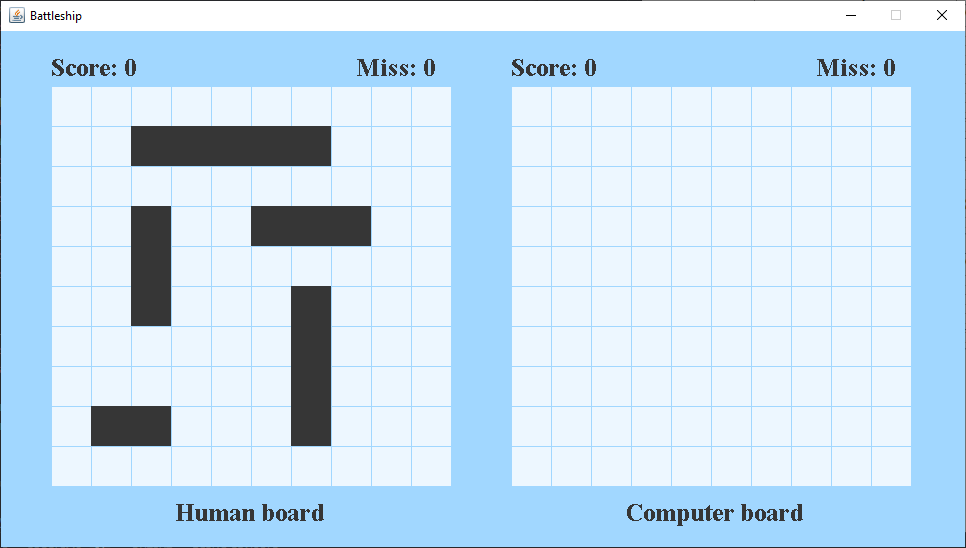
\includegraphics[width=0.7\textwidth]{sources/cap-1.png}
        \caption{Initialisation du plateau}
    \end{figure}

    On clique sur le plateau d'ordinateur pour viser. Quand tous les bateaux sont coulés, le jeu est fini.


\section{Captures d'écran}
\begin{figure}[H]
    \centering
    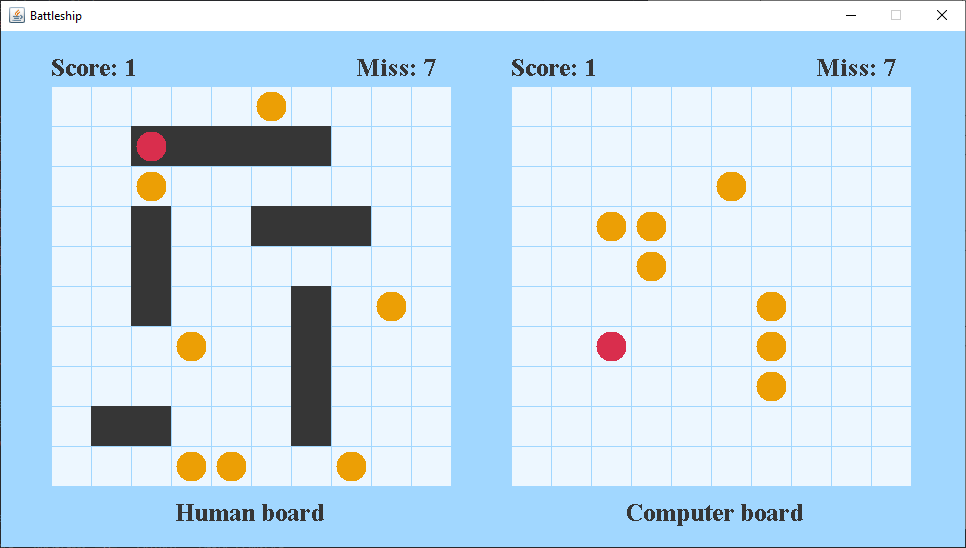
\includegraphics[width=0.7\textwidth]{sources/cap-2.png}
    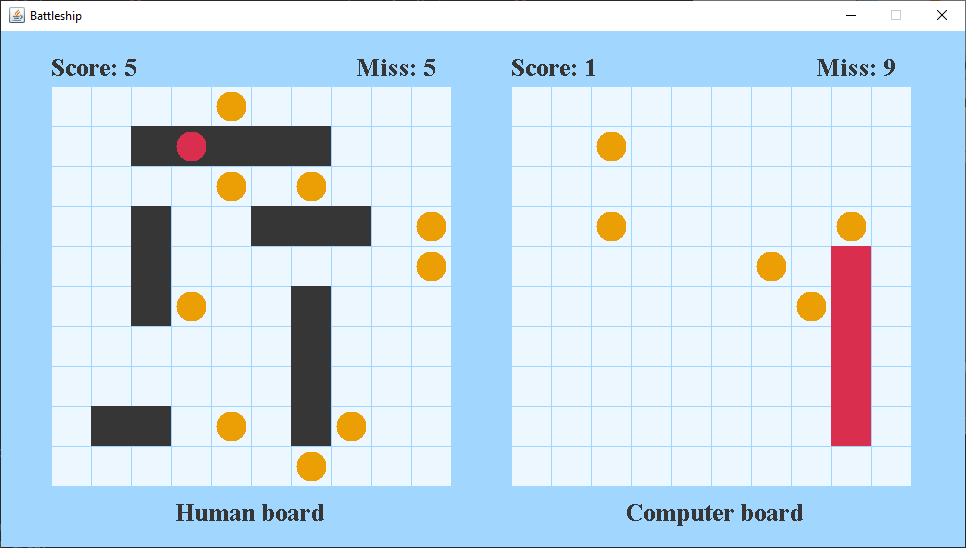
\includegraphics[width=0.7\textwidth]{sources/cap-3.png}
    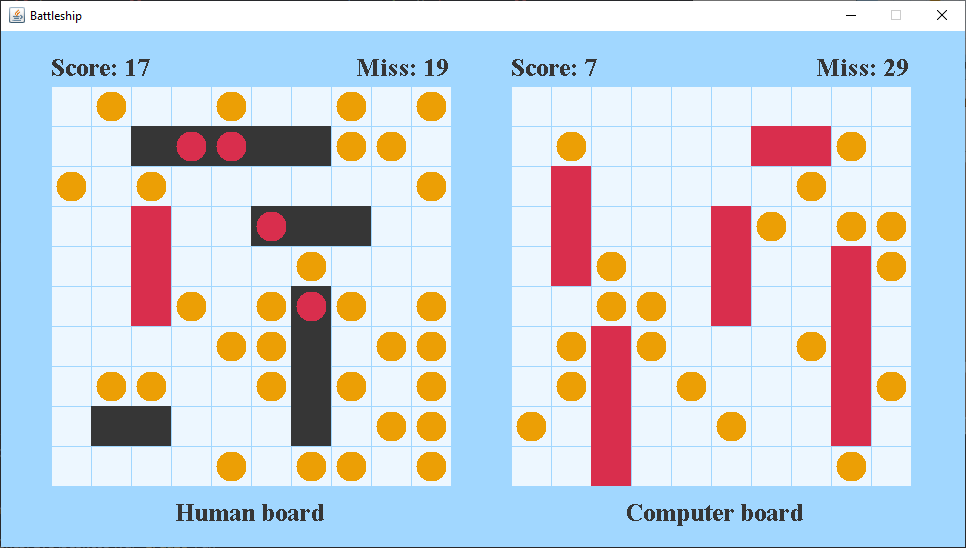
\includegraphics[width=0.7\textwidth]{sources/cap-4.png}
    \caption{Jeu de Bataille Navale}
\end{figure}


\section{Conclusion}
Après ce projet, j'ai mieux compris la libraire Java Swing, le Java Build Tools Gradle, et le jeu de Bataille Navale, je n'ai pas connu ce jeu en précédent. En autre, j'ai avancé la capacité de débugger, d'optimiser le code avec la conception MVC.

Enfin, je veux remercier M. RANAIVOSON de me conseiller pendant les cours de travaux pratiques ainsi que M. MATHET pour ses cours magistraux. Merci d'avoir pris le temps de lire ce rapport.


\bibliographystyle{unsrt}
\bibliography{bibliography}

\end{document}